Le package render (\figurename\ \ref{diagRender}) contient le code de l'interface graphique, c'est-à-dire celui permettant l'affichage du rendu et des fenêtres.

\begin{description}
    \item [MainApp] contient le main de l'application et lance toutes les fenêtres.
    \item [SetSizeWindow] est la classe responsable de la fenêtre du choix de taille du rendu.
    \item [RenderWindow] est la classe responsable de l'affichage de la fenêtre du rendu.
    \item [Toolbox] est la classe responsable de la fenêtre de changement des réglages du rendu en temps réel.
    \item [CameraTimer] est la classe responsable du déplacement de la caméra lors de l'appui de touches du clavier.
    \item [DoImageTask] est la \textit{Task} contenant les calculs du rendu. Voir la section \ref{UsageTask} pour l'usage des tâches.
\end{description}



\begin{figure}[h]
   \begin{center}
       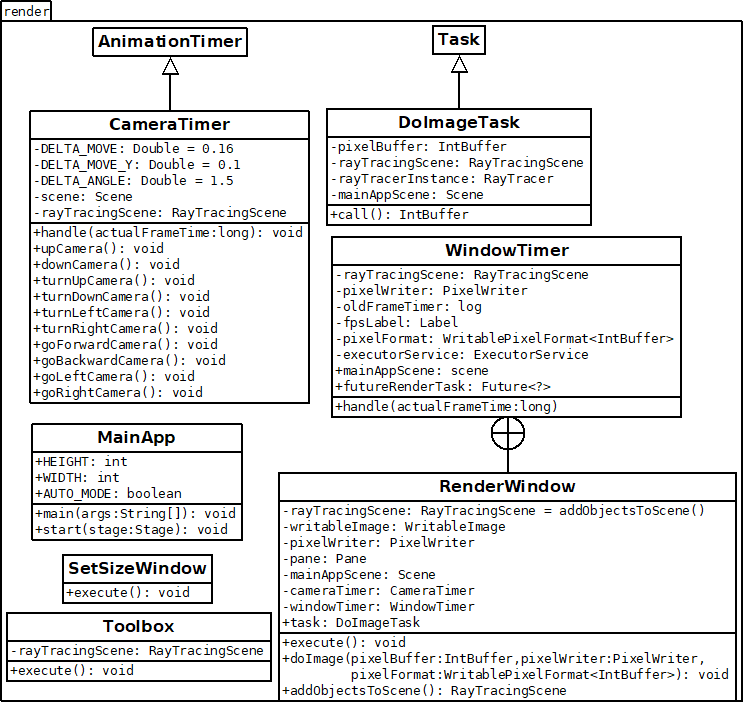
\includegraphics[scale=0.5]{diagrammes/diagClassRender.png}
   \end{center}
   \caption{Diagramme du package render \label{diagRender}}
\end{figure}
\FloatBarrier
